% संपूर्ण मराठी ग्रंथातील प्रकरण 6: अनंत संच
% हा संपादनयोग्य स्रोतखंड आहे. संकलनासाठी संपूर्ण स्रोतसंग्रहातील
% अक्षररूपे, पूर्वभाग, चिन्हव्याख्या आणि आकृती-स्रोत आवश्यक आहेत.
% मूळ: Open Logic Project; मजकूर आणि रूपांतर CC BY 4.0.
% यंत्रानुवाद, दुरुस्ती आणि तपासणी: OpenAI Codex —
% GPT-5.6 Sol आणि GPT-6 Sol, दोन्ही Ultra effort.
% दुरुस्ती-पुनरावलोकन: GPT-6.1 Sol, Ultra effort.
\chapter{अनंत संच}\label{sfr:infinite::chap}
\begin{editorial}
अनंत संचांवरील हे प्रकरण टिम बटन यांच्या \emph{Open Set Theory}
या ग्रंथातून घेतले आहे.
\end{editorial}




\section{हिल्बर्ट यांचे हॉटेल}\label{sfr:infinite:hilbert:sec}

नैसर्गिक संख्यांचा संच स्पष्टपणे अनंत आहे. म्हणून, नैसर्गिक संख्या
स्वतःच \emph{आयत्या गृहीत धरायच्या} नसतील, तर नैसर्गिक संख्यांचा उल्लेख
न करता अनंत संचाचे वैशिष्ट्य सांगणे ही आपली पहिली पायरी असली पाहिजे.
सन 1924 मधील एका व्याख्यानात हिल्बर्ट यांनी मांडलेला पुढील दृष्टिकोन
सुबक आहे. ते आपल्याला अशी कल्पना करायला सांगतात:
\begin{quote}
[\ldots] सांत संख्येने खोल्या असलेले एक हॉटेल. या सर्व खोल्यांपैकी
प्रत्येक खोलीत नेमका एक पाहुणा असावा. आता पाहुण्यांनी कशाही प्रकारे
आपापल्या खोल्या बदलल्या, [पण] प्रत्येक खोलीत अजूनही एकापेक्षा अधिक
व्यक्ती राहणार नाही अशा रीतीने, तर एकही खोली मोकळी होणार नाही आणि
हॉटेलमालकाला या मार्गाने नव्याने येणाऱ्या पाहुण्यासाठी नवी जागा निर्माण
करता येणार नाही [\ldots
\textparagraph \ldots]

आता हॉटेलमध्ये $1$, $2$, $3$, $4$, $5$, \dots अशा क्रमांकांच्या अनंत
खोल्या असतील आणि प्रत्येक खोलीत नेमका एक पाहुणा असेल, असे आपण ठरवू.
नवा पाहुणा येताच मालकाने प्रत्येक जुन्या पाहुण्याला त्याच्या खोलीच्या
क्रमांकापेक्षा एकाने मोठा क्रमांक असलेल्या खोलीत हलवायचे असते; मग नव्याने
आलेल्या पाहुण्यासाठी खोली~$1$ मोकळी होईल.
	\begin{center}
		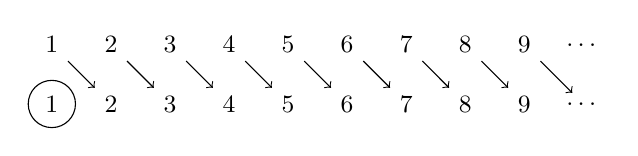
\begin{tikzpicture}[scale = .75]
		\foreach \x in {1, 2, 3, 4, 5, 6, 7, 8, 9}
		{
			\node (\x a) at (\x, 1) {\small{\x}};
			\node (\x b) at (\x, 2) {\small{\x}};
		}
		\node (dotsa) at (10, 1) {\small{\ldots}};
		\node (dotsb) at (10, 2) {\small{\ldots}};
		\draw[->] (1b)--(2a);
		\draw[->] (2b)--(3a);
		\draw[->] (3b)--(4a);
		\draw[->] (4b)--(5a);
		\draw[->] (5b)--(6a);
		\draw[->] (6b)--(7a);
		\draw[->] (7b)--(8a);
		\draw[->] (8b)--(9a);
		\draw[->] (9b)--(dotsa);
		\draw (1,1) circle (.4);
		\end{tikzpicture}
	\end{center}
	(Ewald आणि Sieg (2013, p.~730) मध्ये प्रकाशित; अनुवाद आमचा)
\end{quote}
निर्णायक मुद्दा असा की हिल्बर्ट यांच्या हॉटेलमध्ये अनंत खोल्या आहेत;
आणि असे म्हणण्याचा अर्थ काय, याची व्याख्या म्हणून आपण त्यांचे स्पष्टीकरण
घेऊ शकतो. खरे तर हाच डेडेकिंड यांचा दृष्टिकोन होता (अर्थातच येथे फार
मोठा कालविपर्यास करून तो मांडला आहे; डेडेकिंड यांची व्याख्या
1888 मधील आहे):

\begin{defn}\label{sfr:infinite:hilbert:defn:DedekindInfinite}
संच $A$ हा \emph{डेडेकिंड-अनंत} असतो जर आणि तरच $A$ पासून~$A$ च्या
एखाद्या उचित उपसंचाकडे एकास-एक फलन असते. म्हणजे, असा काही $o \in A$
आणि एकास-एक फलन $f \colon A \to A$ असतात की $o \notin \ran{f}$.
\end{defn}







\section{डेडेकिंड बीजसंरचना}\label{sfr:infinite:dedekind:sec}

नैसर्गिक संख्या केवळ अनंत असाव्यात असेच आपल्याला वाटत नाही; त्यांना काही
(बीजगणितीय) गुणधर्म असावेत असेही आपल्याला वाटते: बेरीज, गुणाकार इत्यादी
क्रियांखाली त्यांनी योग्य रीतीने वागले पाहिजे.

\emph{उत्तरवर्ती फलनाची} कल्पना मूलभूत मानून, पुढील गुणधर्म असलेल्या
वस्तू म्हणजे संख्या असे त्यांचे वैशिष्ट्य सांगावे, ही डेडेकिंड यांची
कल्पना होती:
\begin{enumerate}
	\item अशी $0$ ही संख्या आहे जी कोणत्याही संख्येची उत्तरवर्ती नाही
	\\म्हणजे, $0 \notin \ran{s}$
	\\म्हणजे, $\forall x\ s(x) \neq 0$
	\item भिन्न संख्यांच्या उत्तरवर्ती संख्या भिन्न असतात
	\\म्हणजे, $s$ हे एकास-एक फलन आहे
	\\म्हणजे, $\forall x \forall y (s(x) = s(y) \lif x = y)$
	\item\label{sfr:infinite:dedekind:repeatedapplication} प्रत्येक संख्या $0$ पासून
	उत्तरवर्ती फलन वारंवार लावून मिळते.
\end{enumerate}
पहिल्या दोन अटी प्रथम-क्रम तर्कशास्त्र वापरून सहज हाताळता येतात (वर
पाहा). पण केवळ प्रथम-क्रम तर्कशास्त्र वापरून \ref{sfr:infinite:dedekind:repeatedapplication}
ही अट हाताळता येत नाही. \ref{sfr:infinite:dedekind:repeatedapplication} ही अट पुढीलप्रमाणे
संचसैद्धान्तिक रूपात पुन्हा मांडणे ही डेडेकिंड यांची निर्णायक कामगिरी होती:
\begin{enumerate}
	\item[3$'$.] नैसर्गिक संख्यांचा संच हा \emph{उत्तरवर्ती फलनाखाली
	बंद} असलेला लघुतम संच आहे: म्हणजे, संचातील कोणत्याही घटक वर
	$s$ लावल्यास संचातीलच दुसरा घटक मिळतो.
\end{enumerate}
पण हे आपल्याला सावकाश आणि स्पष्टपणे मांडावे लागेल.

\begin{defn}\label{sfr:infinite:dedekind:Closure}
	कोणत्याही फलन $f$ साठी, संच $X$ हा $f$-\emph{बंद} असतो जर आणि तरच
	$(\forall x \in X)f(x) \in X$. आता कोणत्याही $o$ साठी अशी व्याख्या करू:
	$$\closureofunder{f}{o} = \bigcap\Setabs{X}{o \in X\text{ आणि }X
\text{ हा $f$-बंद आहे}}$$
\end{defn}

म्हणून $\closureofunder{f}{o}$ हा $o$ हा घटक असलेल्या सर्व
$f$-बंद संचांचा छेद आहे. त्यामुळे सहजज्ञानानुसार,
$\closureofunder{f}{o}$ हा $o$ हा घटक असलेला \emph{लघुतम}
$f$-बंद संच आहे. पुढील निष्कर्ष हे सहजज्ञान नेमकेपणाने मांडतो:
\begin{lem}\label{sfr:infinite:dedekind:closureproperties}
	कोणतेही फलन $f$ आणि कोणतेही $o \in A$ यांसाठी:
	\begin{enumerate}
		\item\label{sfr:infinite:dedekind:closurehaselem} $o \in \closureofunder{f}{o}$; आणि
		\item\label{sfr:infinite:dedekind:closureclosed} $\closureofunder{f}{o}$ हा $f$-बंद आहे; आणि
		\item\label{sfr:infinite:dedekind:closuresmallest} $X$ हा $f$-बंद असून $o \in
		X$ असेल, तर $\closureofunder{f}{o} \subseteq X$
	\end{enumerate}
\end{lem}

\begin{proof}
$o$ हा घटक असलेला किमान एक $f$-बंद संच आहे, हे लक्षात घ्या;
तो म्हणजे $\ran{f}\cup \{o\}$. म्हणून अशा \emph{सर्व} संचांचा छेद
$\closureofunder{f}{o}$ अस्तित्वात आहे. आता आपल्याला
\ref{sfr:infinite:dedekind:closurehaselem}--\ref{sfr:infinite:dedekind:closuresmallest} तपासावे लागतील.

\ref{sfr:infinite:dedekind:closurehaselem} बाबत: छेदातील सर्व संचांत $o$ हा घटक
असल्यामुळे $o \in \closureofunder{f}{o}$.

\ref{sfr:infinite:dedekind:closureclosed} बाबत: $x \in \closureofunder{f}{o}$ असे समजा.
म्हणून $o \in X$ आणि $X$ हा $f$-बंद असेल, तर $x \in X$; आणि $X$ हा
$f$-बंद असल्यामुळे $f(x) \in X$. म्हणून
$f(x) \in \closureofunder{f}{o}$.

\ref{sfr:infinite:dedekind:closuresmallest} बाबत: सर्वसाधारणपणे, $X \in C$ असेल, तर
$\bigcap C \subseteq X$.
\end{proof}

याचा उपयोग करून आपण असे म्हणू शकतो:

\begin{defn}
संच $A$, फलन $f \colon A \to A$ आणि असा काही $o \in A$ यांनी मिळून
\emph{डेडेकिंड बीजसंरचना} बनते, जर:
	\begin{enumerate}
		\item \label{sfr:infinite:dedekind:ded:proper} $o \notin \ran{f}$
		\item \label{sfr:infinite:dedekind:ded:injection} $f$ हे एकास-एक फलन आहे
		\item \label{sfr:infinite:dedekind:ded:closure} $A = \closureofunder{f}{o}$
	\end{enumerate}
\end{defn}

$A = \closureofunder{f}{o}$ असल्यामुळे, आधीच्या निष्कर्षावरून $A$ हा
$o$ हा घटक असलेला लघुतम $f$-बंद संच आहे. डेडेकिंड बीजसंरचना
स्पष्टपणे डेडेकिंड-अनंत असते; व्याख्येतील \ref{sfr:infinite:dedekind:ded:proper} आणि
\ref{sfr:infinite:dedekind:ded:injection} ही कलमे पाहा. पण कोणत्याही डेडेकिंड-अनंत संचाचे
डेडेकिंड बीजसंरचनेत रूपांतर करता येते, ही अधिक रोचक गोष्ट आहे.

\begin{thm}\label{sfr:infinite:dedekind:thm:DedekindInfiniteAlgebra}
डेडेकिंड-अनंत संच अस्तित्वात असेल, तर डेडेकिंड बीजसंरचना अस्तित्वात असते.
\end{thm}

\begin{proof}
$D$ हा डेडेकिंड-अनंत असू द्या. मग एकास-एक फलन $g \colon D \to D$
आणि घटक $o  \in D \setminus \ran{g}$ अस्तित्वात आहेत. आता $A =
\closureofunder{g}{o}$ असे मानू; \ref{sfr:infinite:dedekind:closureproperties} नुसार $A$
अस्तित्वात आहे आणि $o \in A$. $f = \funrestrictionto{g}{A}$ असे मानू.
$A, f, o$ हे मिळून डेडेकिंड बीजसंरचना बनतात, हे आपण दाखवू.

\ref{sfr:infinite:dedekind:ded:proper} बाबत: $o \notin \ran{g}$ आणि $\ran{f}
\subseteq \ran{g}$, म्हणून $o\notin \ran{f}$.

\ref{sfr:infinite:dedekind:ded:injection} बाबत: $g$ हे $D$ वरील एकास-एक फलन आहे; म्हणून
$f \subseteq g$ हेही एकास-एक फलन असले पाहिजे.

\ref{sfr:infinite:dedekind:ded:closure} बाबत: \ref{sfr:infinite:dedekind:closureproperties} नुसार $A$ हा
$g$-बंद आहे; त्यामुळे विशेषतः $A$ हा $f$-बंद आहे. म्हणून
\ref{sfr:infinite:dedekind:closureproperties} नुसार $\closureofunder{f}{o} \subseteq A$.
तसेच $\closureofunder{f}{o}$ हा $f$-बंद आहे आणि
$f = \funrestrictionto{g}{A}$ असल्यामुळे $\closureofunder{f}{o}$ हा
$g$-बंद आहे. म्हणून \ref{sfr:infinite:dedekind:closureproperties} नुसार
$A \subseteq \closureofunder{f}{o}$.
\end{proof}








\section{डेडेकिंड बीजसंरचना आणि अंकगणितीय विगमन}\label{sfr:infinite:induction:sec}

आता निर्णायक बाब अशी की एखादी डेडेकिंड बीजसंरचना---खरे तर,
\emph{कोणतीही} डेडेकिंड बीजसंरचना---नैसर्गिक संख्यांचे पर्यायी प्रतिरूप
म्हणून उपयोगी पडेल. हे पुढील सहज निष्पत्तीमुळे घडते:

\begin{thm}[अंकगणितीय विगमन]\label{sfr:infinite:induction:thm:dedinfiniteinduction}
$N, s, o$ यांनी मिळून डेडेकिंड बीजसंरचना बनते असे समजा. मग कोणत्याही
संच $X$ साठी:
	\begin{center}
		जर $o \in X$ आणि $(\forall {n} \in N \cap X){s}({n}) \in X$, {तर} $N \subseteq X$.
	\end{center}
\end{thm}

\begin{proof}
डेडेकिंड बीजसंरचनेच्या व्याख्येनुसार $N = \closureofunder{s}{o}$.
आता ${o} \in X$ आणि $(\forall {n} \in N)(n \in X \lif
{s}({n}) \in X)$ या दोन्ही अटी पूर्ण होत असतील, तर
$N = \closureofunder{s}{o} \subseteq X$.
\end{proof}

विगमन हा नैसर्गिक संख्यांचा वैशिष्ट्यपूर्ण गुणधर्म असल्यामुळे मुद्दा असा
आहे: कोणताही डेडेकिंड-अनंत संच दिला असता, आपण डेडेकिंड बीजसंरचना बनवू
शकतो आणि ती बीजसंरचना नैसर्गिक संख्यांचे पर्यायी प्रतिरूप म्हणून वापरू
शकतो.

हे मान्यच की \ref{sfr:infinite:induction:thm:dedinfiniteinduction} मध्ये विगमन
\emph{संचसैद्धान्तिक} भाषेत मांडले आहे. पण हे तत्त्व अधिक परिचित वाटेल
अशा भाषेत आपण सहज मांडू शकतो:

\begin{cor}\label{sfr:infinite:induction:natinductionschema}
$N, s, o$ यांनी मिळून डेडेकिंड बीजसंरचना बनते असे समजा. मग प्राचले असू
शकतील अशा कोणत्याही सूत्र $\phi(x)$ साठी:
\begin{center}
	जर $\phi(o)$ आणि $(\forall {n} \in N)(\phi(n)\lif
	\phi({s}({n})))$, {तर} $(\forall n \in N)\phi(n)$
\end{center}
\end{cor}

\begin{proof}
$X = \Setabs{n \in N}{\phi(n)}$ असे मानून आता
\ref{sfr:infinite:induction:thm:dedinfiniteinduction} वापरा.
\end{proof}

या निष्कर्षात आपण सूत्राला ``प्राचले असण्याबद्दल'' बोललो. याचा ढोबळ
अर्थ असा की कोणत्याही वस्तू $c_1, \ldots, c_k$ साठी आपण
$\phi(x, c_1, \ldots, c_k)$ बरोबर काम करू शकतो. अधिक नेमकेपणाने,
``प्राचले'' असा उल्लेख न करता निष्कर्ष पुढीलप्रमाणे मांडता येतो.
ज्याची सर्व मुक्त चरे दाखवली आहेत अशा कोणत्याही सूत्र
$\phi(x, v_1, \ldots, v_k)$ साठी:
	\begin{align*}
			\forall v_1 \ldots \forall v_k((&\phi(o, v_1,\ldots, v_k) \land {}\\
			&	(\forall x \in N)(\phi(x,v_1, \ldots, v_k) \lif \phi(s(x), v_1,\ldots, v_k))) \lif {}\\
			&\hspace{3em} (\forall x \in N)\phi(x, v_1,\ldots, v_k))
	\end{align*}
``प्राचले असणे'' असे म्हणाल्याने मजकूर वाचणे फारच सोपे होते, हे उघड आहे.
(पर्यायी विभाग मध्ये आपण ही युक्ती वारंवार वापरू.)

पुन्हा डेडेकिंड बीजसंरचनांकडे वळू: कोणतीही डेडेकिंड बीजसंरचना दिली
असता, बेरीज, गुणाकार आणि घातांक क्रिया यांची नेहमीची अंकगणितीय फलनेही
आपण परिभाषित करू शकतो. मात्र हे क्षुल्लक नाही आणि त्यात
\emph{पुनरावर्ती व्याख्येचे} तंत्र वापरावे लागते. हे तंत्र आपण बरेच नंतर,
त्यापेक्षा अधिक व्यापक संदर्भात मांडू आणि समर्थित करू.
(उत्सुक वाचकांनी पर्यायी विभाग नंतर याकडे पुन्हा
वळावे किंवा Potter (2004, pp.~95--8) यांसारखा पर्यायी विवेचनग्रंथ
वाचावा.) पण $N, s, o$ यांनी डेडेकिंड बीजसंरचना बनत असेल, तर शेवटी
आपल्याला पुढीलप्रमाणे अर्थ ठरवता येईल:
\begin{align*}
	{a} + {o} &= {a} & & & {a} \times {o} &= {o} & & & {a}^{o} &= s(o)\\
{a} + {s}({b}) &= {s}({a}+{b}) &&& {a} \times {s}({b}) &= ({a}\times {b}) + {a}  & & & {a}^{{s}({b})} &= {a}^{b} \times {a}
\end{align*}
आणि ही फलने आपल्या अपेक्षेप्रमाणे वागतात, हे दाखवता येईल.









\section{अनंत संचाच्या अस्तित्वाची
डेडेकिंड यांची ``सिद्धता''}\label{sfr:infinite:dedekindsproof:sec}

या प्रकरणात आपण डेडेकिंड बीजसंरचनांच्या साहाय्याने नैसर्गिक संख्यांचे
संचसैद्धान्तिक विवेचन दिले. \ref{sfr:arith:ref:sec} मध्ये आपण इतर
गोष्टींबरोबर विश्लेषणाच्या अंकगणितीकरणाच्या तात्त्विक महत्त्वाचा विचार
केला. आता येथे आपण जे साध्य केले आहे त्याच्या महत्त्वाचा विचार करायला हवा.

संपूर्ण \ref{sfr:arith::chap} मध्ये आपण नैसर्गिक संख्या आयत्या
मानल्या आणि त्यांचा वापर करून पूर्णांक, परिमेय संख्या आणि वास्तव संख्या
यांची स्पष्ट रचना केली. या प्रकरणात आपण नैसर्गिक संख्यांची स्पष्ट रचना
दिलेली नाही. आपण एवढेच दाखवले आहे की \emph{कोणताही डेडेकिंड-अनंत संच
दिला असता}, आपण असा संच परिभाषित करू शकतो जो आपल्याला~$\Nat$ ने जसे
वागावेसे वाटते अगदी तसाच वागेल.

त्यामुळे \emph{कोणत्या वस्तू नैसर्गिक संख्या आहेत} अशा सत्तामीमांसक
प्रश्नाचे उत्तर आपण दिले आहे, असा दावा अर्थातच करता येणार नाही. पण ही
चांगलीच गोष्ट आहे. शेवटी, \ref{sfr:arith:ref:sec} मध्ये आपण यावर
भर दिला होता की $\Real$ म्हणजे डेडेकिंड छेदांचा संच ही व्याख्या सोयीची
संकेतजनक व्याख्या न मानता \emph{शोध} मानणे चुकीचे ठरेल. डेडेकिंड छेद
वास्तव संख्यांच्या प्रमुख गणितीय गुणधर्मांचे उदाहरण देतात, हे निर्णायक
निरीक्षण आहे. येथेही तसेच: \emph{कोणतीही} डेडेकिंड बीजसंरचना नैसर्गिक
संख्यांच्या प्रमुख गणितीय गुणधर्मांचे उदाहरण देते, हे निर्णायक निरीक्षण
आहे. (खरे तर सर्व डेडेकिंड बीजसंरचना परस्पर \emph{समरूपी} आहेत, हे
सिद्ध करून डेडेकिंड यांनी हा मुद्दा ठामपणे दाखवला
(1888, प्रमेये 132--3). त्यामुळे आजचे अनेक
``संरचनावादी'' डेडेकिंड यांना पूर्वसूरी मानतात, यात आश्चर्य नाही.)

 शिवाय आपण नैसर्गिक संख्यांचा सिद्धान्त अशा अनौपचारिक साध्या
 संचसिद्धान्तात कसा अंतःस्थापित करायचा हे दाखवले आहे, जो स्वतः अजूनही
 बराच अनौपचारिक आहे, पण नैसर्गिक संख्या आयत्या गृहीत धरत नाही असे
 (वरवर तरी) दिसते. त्यामुळे डेडेकिंड यांचा स्वतःचा महत्त्वाकांक्षी
 प्रकल्प प्रत्यक्षात आणण्याच्या मार्गावर आपण असू शकतो. त्यांनी तो असा
 स्पष्ट केला:
\begin{quote}
	विज्ञानात सिद्ध करण्याजोगी कोणतीही गोष्ट सिद्धतेशिवाय मान्य करू नये.
	ही मागणी रास्त वाटत असली, तरी अगदी साध्या विज्ञानाचा पाया घालण्याच्या
	सर्वांत अलीकडील पद्धतींमध्येही ती पूर्ण झाली आहे असे मला मानता येत
	नाही; म्हणजे, संख्यासिद्धान्ताशी संबंधित तर्कशास्त्राच्या त्या भागातही.
	अंकगणित (बीजगणित, विश्लेषण) हे तर्कशास्त्राचाच केवळ एक भाग आहे असे
	म्हणताना माझा आशय असा की संख्या ही संकल्पना अवकाश आणि काळ यांच्या
	कल्पना किंवा अंतःप्रज्ञा यांपासून पूर्णपणे स्वतंत्र आहे---ती विचारांच्या
	शुद्ध नियमांचे थेट फलित आहे असेच मी मानतो.
	(Dedekind, 1888, प्रस्तावना)
\end{quote}
डेडेकिंड यांची धाडसी कल्पना अशी आहे. आपण नुकतेच पाहिले की केवळ
(अनौपचारिक) संचसिद्धान्त वापरून नैसर्गिक संख्या कशा घडवायच्या.
\ref{sfr:arith::chap} मध्ये आपण पाहिले की नैसर्गिक संख्या आणि काही
संचसिद्धान्त दिला असता वास्तव संख्यांची रचना कशी करायची. त्यामुळे कदाचित
``अंकगणित (बीजगणित, विश्लेषण)'' हे ``तर्कशास्त्राचाच केवळ एक भाग'' ठरते
(डेडेकिंड यांच्या ``तर्कशास्त्र'' या शब्दाच्या विस्तारित अर्थाने).

ही झाली कल्पना. पण क्षणभर थांबा. डेडेकिंड बीजसंरचनेची आपली रचना
(म्हणजे नैसर्गिक संख्यांचे आपले पर्यायी प्रतिरूप) डेडेकिंड-अनंत संचाच्या
अस्तित्वावर अवलंबून आहे. (मागे \ref{sfr:infinite:dedekind:thm:DedekindInfiniteAlgebra}
पाहा.) डेडेकिंड-अनंत संचाचे अस्तित्व ``तर्कशास्त्र'' किंवा ``विचारांचे
शुद्ध नियम'' यांच्या साहाय्याने प्रस्थापित करता आले नाही, तर हा प्रकल्प
अडून पडतो.

मग डेडेकिंड-अनंत संचाचे अस्तित्व ``विचारांच्या शुद्ध नियमांनी''
प्रस्थापित \emph{करता येते का}? डेडेकिंड यांचा प्रयत्न असा होता:
\begin{quote}
  माझे स्वतःचे विचारविश्व, म्हणजे माझ्या विचारांचे विषय होऊ शकणाऱ्या सर्व
  वस्तूंची समग्रता $S$, अनंत आहे. कारण $s$ हा~$S$ चा घटक दर्शवत असेल,
  तर $s$ हा माझ्या विचाराचा विषय होऊ शकतो हा विचार $s'$ स्वतः~$S$ चा
  घटक आहे. याला घटक~$s$ ची प्रतिमा $\phi(s)$ मानले, तर
  \dots~$S$ हा [डेडेकिंडच्या अर्थाने] अनंत आहे, हेच सिद्ध करायचे होते.
	(Dedekind, 1888, \S66)
\end{quote}
मुख्यतः अत्यंत काटेकोर गणितीय सिद्धतांनी भरलेल्या ग्रंथाच्या मध्यभागी
अशी गोष्ट सापडणे खरोखरच चकित करणारे आहे. येथे दोन टिप्पण्या कराव्याशा
वाटतात.

पहिली: या ``सिद्धतेला'' आज आपण ``गणितीय'' स्वरूप म्हणून ओळखू असे स्वरूप
जवळजवळ नाहीच. ती मानसशास्त्रीय वस्तूंबद्दल (विचारांबद्दल) बोलते आणि
त्यातही केवळ \emph{संभाव्य} विचारांबद्दल बोलते.

दुसरी: निदान आपण डेडेकिंड बीजसंरचना ज्या रीतीने मांडल्या आहेत त्या
रीतीनुसार, या ``सिद्धतेत'' एक सरळ तांत्रिक उणीव आहे. डेडेकिंड यांचा
युक्तिवाद यशस्वी झाला, तरी तो केवळ अनंत वस्तू (विशेषतः अनंत विचार)
अस्तित्वात आहेत एवढेच प्रस्थापित करतो. पण~$S$ ला अनेक घटक असलेला
एकच \emph{संच} का मानावे,~$S$ ला केवळ \emph{काही वस्तू} (अनेकवचनात) का मानू
नये, याचे कारणही डेडेकिंड यांनी द्यायला हवे.

डेडेकिंड यांना येथे उणीव दिसली नाही, यावरून कदाचित त्यांनी वापरलेला
``समग्रता'' हा शब्द \emph{आपण} वापरत असलेल्या ``संच'' या शब्दाशी
तंतोतंत जुळत नाही असे सूचित होते.\footnote{तसे तो जुळत नव्हता असे
मानण्याची इतर कारणेही आपल्याकडे आहेत; पाहा Potter (2004, p.~23).}
पण हे फार आश्चर्यकारक ठरणार नाही. मागील दोन प्रकरणांत आपण राबवलेला
प्रकल्प---नैसर्गिक संख्यांची ``रचना'' आणि त्यांच्यापासून पूर्णांक,
वास्तव संख्या व परिमेय संख्या यांची ``रचना''---संपूर्णपणे अनौपचारिक
रीतीने राबवला आहे. नेमके कोणते संच कधी अस्तित्वात असतात याविषयी अनेक
सामान्य तत्त्वे न मांडता, गरज पडेल तेव्हा आपण हा संच किंवा तो संच आयता
मानला. पण काही सामान्य तत्त्वांची आपल्याला \emph{गरज} आहे हे माहीत आहे;
नाहीतर आपल्याला रसेलच्या विरोधापत्तीला सामोरे जावे लागेल.

 आता अनौपचारिकतेच्या या मर्यादा ओलांडण्याची वेळ आली आहे.








\section{परिशिष्ट: श्रेडर--बर्नस्टाइनची सिद्धता}\label{sfr:infinite:card-sb:sec}

अनौपचारिक संचसिद्धान्ताचा निरोप घेण्यापूर्वी, आणखी एका अनौपचारिक
(पण प्रगत!) सिद्धतेचा विचार करायचा आहे. ही श्रेडर--बर्नस्टाइनची सिद्धता
आहे (\ref{sfr:siz:sb:thm:schroder-bernstein}): जर
$\cardle{A}{B}$ आणि $\cardle{B}{A}$, तर $\cardeq{A}{B}$; म्हणजे,
एकास-एक फलने $f \colon A \to B$ आणि $g \colon B \to A$ दिली असता
एकास-एक आच्छादन $h \colon A \to B$ असते.

या प्रकरणात आपण डेडेकिंड यांच्या \emph{संवरणांच्या} संकल्पनेचा वापर
केला. किंबहुना याच संकल्पनेचा उपयोग करून डेडेकिंड यांनी
श्रेडर--बर्नस्टाइनची एक सुंदर सिद्धता दिली; ती येथे मांडू. ही सिद्धता
Potter (2004, pp.~157--8) यांच्या विवेचनाला अगदी जवळून अनुसरते;
तेथील मांडणी किंचित वेगळी पण मूलतः समान आहे. इंटरनेटवर थोडा शोध
घेतल्यास असेही दिसेल की---$\sqrt{2}$ च्या अपरिमेयतेप्रमाणेच---या
प्रमेयाच्या \emph{अनेक} रोचक आणि वेगवेगळ्या सिद्धता आहेत.

\ref{sfr:infinite:dedekind:Closure} मधील संकेतनासारखेच संकेतन
वापरून, प्रत्येक संच $B$ आणि फलन~$f$ यांसाठी
\[\Closureofunder{f}{B} = \bigcap \Setabs{X}{B \subseteq X
\text{ आणि $X$ हा $f$-बंद आहे}}
\]
असे मानू. अशा रीतीने परिभाषित केलेला $\Closureofunder{f}{B}$ हा~$B$
चा समावेश असलेला लघुतम $f$-बंद संच आहे; म्हणजे:

\begin{lem}\label{sfr:infinite:card-sb:Closureprops}
	कोणतेही फलन $f$ आणि कोणताही $B$ यांसाठी:
	\begin{enumerate}
		\item\label{sfr:infinite:card-sb:Closurehaselem} $B \subseteq \Closureofunder{f}{B}$; आणि
		\item\label{sfr:infinite:card-sb:Closureclosed} $\Closureofunder{f}{B}$ हा $f$-बंद आहे; आणि
		\item\label{sfr:infinite:card-sb:Closuresmallest} $X$ हा $f$-बंद असून $B
		\subseteq X$ असेल, तर $\Closureofunder{f}{B} \subseteq X$.
	\end{enumerate}
\end{lem}

\begin{proof}
\ref{sfr:infinite:dedekind:closureproperties} मधील सिद्धतेप्रमाणेच.
\end{proof}

श्रेडर--बर्नस्टाइनपर्यंत पोहोचण्यासाठी आपल्याला आणखी एका तथ्याची गरज आहे:

\begin{prop}\label{sfr:infinite:card-sb:sbhelper}
जर $A \subseteq B \subseteq C$ आणि $A \approx C$, तर $\cardeq{B}{C}$.
\end{prop}
\begin{quote}\small\textbf{स्रोतदुरुस्ती.} MRINF-003 पात्रता: गोठवलेल्या इंग्रजीतील अंतःस्थ cardeq रचना $A\approx B\approx C$ अशी वैध रीतीने विस्तारते; ती स्रोतदोष नाही. मराठीतील स्पष्ट $B\approx C$ निष्कर्ष त्याच तुल्यबलता-साखळीतील, पुढील उपयोगासाठी केंद्रित केलेली सममूल्य मांडणी आहे.\end{quote}

\begin{proof}
एकास-एक आच्छादन  $f \colon C \to A$ दिले असता, $F =
\Closureofunder{f}{C \setminus B}$ असे मानू आणि प्रांत $C$ असलेले फलन
$g$ पुढीलप्रमाणे परिभाषित करू:
\[	g(x) =
	\begin{cases}
			f(x) &\text{जर $x \in F$}\\
			x & \text{अन्यथा}
	\end{cases}
\]
$g$ हे $C \to B$ असे एकास-एक आच्छादन आहे, हे आपण दाखवू. त्यावरून
$\comp{f^{-1}}{g} \colon A \to B$ हे एकास-एक आच्छादन आहे आणि सिद्धता
पूर्ण होते.

प्रथम आपला दावा असा आहे की $x \in F$ पण $y\notin F$ असेल, तर $g(x) \neq
g(y)$. विरोधाभासाने सिद्ध करण्यासाठी तसे नाही असे समजा; मग $y = g(y) =
g(x) = f(x)$. $x \in F$ आहे आणि \ref{sfr:infinite:card-sb:Closureprops} नुसार $F$ हा
$f$-बंद आहे, म्हणून $y = f(x) \in F$; हा विरोधाभास आहे.

आता $g(x) = g(y)$ असे समजा. वरील दाव्यानुसार, $x \in F$ तेव्हा आणि
केवळ तेव्हाच, जेव्हा $y \in F$. जर $x, y \in F$, तर $f(x) = g (x) =
g(y) = f(y)$; आणि $f$ हे एकास-एक आच्छादन असल्यामुळे $x = y$. जर
$x, y \notin F$, तर $x = g(x) = g(y) = y$. म्हणून $g$ हे
एकास-एक फलन आहे.

$\ran{g} = B$ हे दाखवणे उरते. म्हणून $x \in B \subseteq C$ स्थिर करू.
जर $x \notin F$, तर $g(x) = x$. जर $x \in F$, तर कोणत्यातरी
$y \in F$ साठी $x = f(y)$; कारण तसे नसते, तर $F \setminus \{x\}$ हा
$f$-बंद संच असता आणि त्यात $C\setminus B$ चा समावेश असता; पण
\ref{sfr:infinite:card-sb:Closureprops} नुसार हे अशक्य आहे. आता $g(y) = f(y) = x$.
\end{proof}

शेवटी, मुख्य निष्कर्षाची सिद्धता पुढीलप्रमाणे. फलन $h$ आणि संच $D$ दिले
असता आपण $\funimage{h}{D} = \Setabs{h(x)}{x \in D}$ अशी व्याख्या करतो,
हे आठवा.

\begin{proof}[श्रेडर--बर्नस्टाइनची सिद्धता] $f \colon A \to B$
आणि $g \colon B \to A$ ही एकास-एक फलने असू द्या.
$\funimage{f}{A} \subseteq B$ असल्यामुळे
$\funimage{g}{\funimage{f}{A}} \subseteq g[B] \subseteq A$.
तसेच, $\comp{f}{g} \colon A \to
\funimage{g}{\funimage{f}{A}}$ हे एकास-एक फलन आहे, कारण $g$ आणि
$f$ दोन्ही तशी आहेत; आणि त्याचा सहप्रांत ज्या रीतीने परिभाषित केला आहे,
त्यावरून $\comp{f}{g}$ हे खरे तर एकास-एक आच्छादन आहे. म्हणून
$\cardeq{\funimage{g}{\funimage{f}{A}}}{A}$; आणि त्यामुळे
\ref{sfr:infinite:card-sb:sbhelper} नुसार $h \colon A \to \funimage{g}{B}$ असे
एकास-एक आच्छादन आहे. शिवाय, $g^{-1}$ हे
$\funimage{g}{B} \to B$ असे एकास-एक आच्छादन आहे. म्हणून
$\comp{h}{g^{-1}} \colon A \to B$ हे एकास-एक आच्छादन आहे.
\end{proof}



